% Definition des noms de la fonction
\newcommand{\frenchname}{Fonction de production de Morel-Seytoux}
\newcommand{\englishname}{Morel-Seytoux production function}
\newcommand{\VersionNumber}{11.5}

% FileID
\newcommand{\FileID}{water.surf-uz.runoff-infiltration.mseytoux}

% Produced variables
\newcommand{\VarProdA}{water.surf.H.runoff}
\newcommand{\VarProdB}{water.surf.H.infiltration}

% Used variables (if necessary)
\newcommand{\VarUsedA}{water.surf.Q.downstream-su}
\newcommand{\VarUsedB}{soil.surf.hydraulic-conductivity-Ks}

% Required variables
\newcommand{\VarRequirA}{water.atm-surf.H.rain}

% Initial conditions
\newcommand{\InitA}{thetaini}

% Parameters
\newcommand{\ParamA}{resstep}
\newcommand{\ParamB}{CoeffMultiKs}
\newcommand{\ParamC}{CoeffMultiThetaIni}


% Attributes
\newcommand{\PropDisB}{thetares}
\newcommand{\PropDisC}{thetasat}
\newcommand{\PropDisD}{betaMS}
\newcommand{\PropDisE}{Hc}
\newcommand{\PropDisF}{area}
\newcommand{\PropDisA}{ks}

% Main file for function description and utilisation
%\selectlanguage{english}

\begin{abstract}
\iflanguage{english}{The rain is separated by the ``\englishname'' into infiltration and runoff on each SU. The function computes the time before all the rain is infiltrated. This caracteristic time is called ``ponding time'' $t_p$. When the ponding time is reached, the function calculates the soil infiltrability using the hydraulic conductivity and the initial soil water content and deduces the runoff. This model is adapted to the \textbf{simulation at the event scale}.}
  {La ``\frenchname`` sépare la pluie en infiltration et ruissellement sur chaque SU. Elle calcule le ''temps de flaquage`` avant lequel toute la pluie s'infiltre dans le sol. Dès que le temps de flaquage $t_p$ est atteint la fonction calcule l'infiltratbilité du sol selon la conductivité à saturation et la teneur initiale en eau du sol et en déduit le ruissellement. L'utilisation de cette fonction est réservée à la simulation à l'\textbf{échelle de l'événement pluvieux}.}
\end{abstract}

%******************************
% Scientific concepts
\iflanguage{english}{\section{Scientific concepts}}{\section{Concepts scientifiques}}
\iflanguage{english}{\subsection{Calculation of water height}
First, the function computes the water height present at the top of the surface unit. This value is composed with rainfall height $P$ (in $m$) and runoff output discharge $Q_{SU}(t-1)$ (in $m\up3/s$) from potential upper connected SUs calculated at the previous simulation time step.

\begin{equation}
\label{HeightSU}
H = P + \sum_{SU_{up}} \left( \frac{Q_{SU}(t-1) \times \Delta t}{A_{SU}} \right)
\end{equation}


where $H$ is the water height present at the surface of the SU ($m$), $\Delta t$ is the simulation time step ($s$), and $A_{SU}$ is the area of the unit on which the calculation is done ($m\up2$).


\subsection{Calculation of infiltrability}
The ``\englishname'' \cite{MorelS1978} is a modification of Green and Ampt's \cite{Green1911} equation. The main assumption is the rectangular form of the wetting front trough the soil, as schematized hereafter. Then, the model was adapted to the MHYDAS structure by Moussa and al. \cite{Moussa2002}.\\

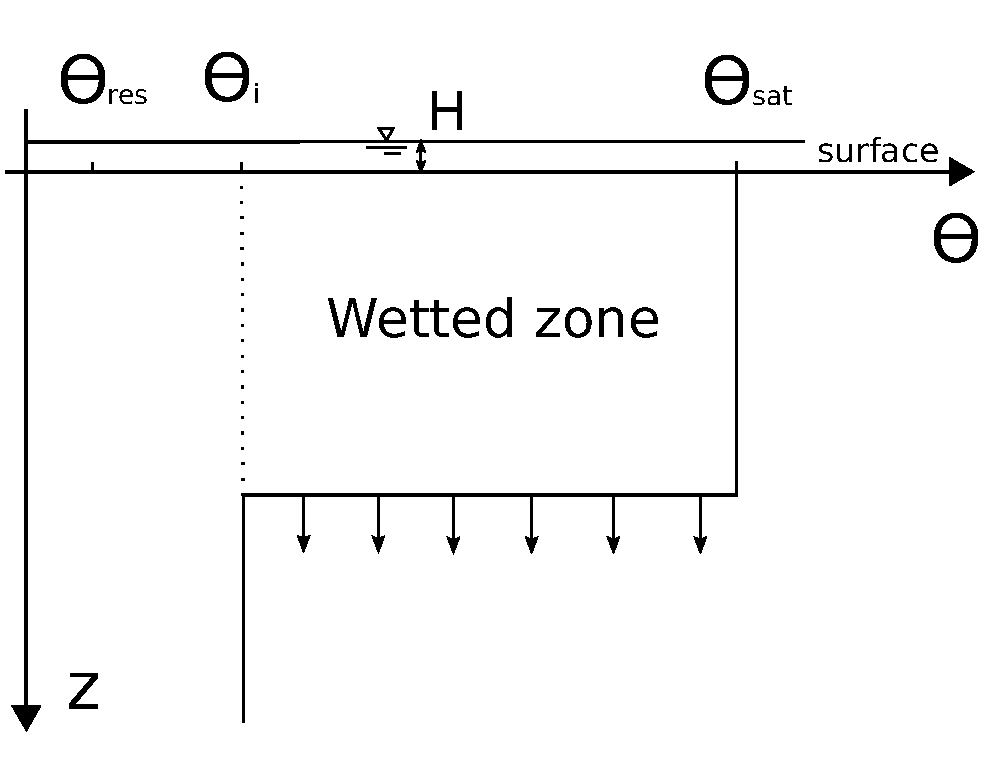
\includegraphics[width=8cm]{common/Green_Ampt_humidity.pdf}

Runoff cannot occur as long as the soil surface retention potential is not reached. Therefore, at every time step, the model needs to determine whether the ponding time ($t_p$) has been reached. For $t < t_p$ all the rain is infiltrated and for $t > t_p$ the cumulative infiltration $F(t)$ is calculated from the equation \ref{MSeytoux}. This behaviour could be represented with the infiltratbility $f(t)$ ($m/s$) which dicrease in time from $t_p$. Then, the value of $f(t)$ tends towards the saturated hydraulic conductivity $K_{sat}$.\\

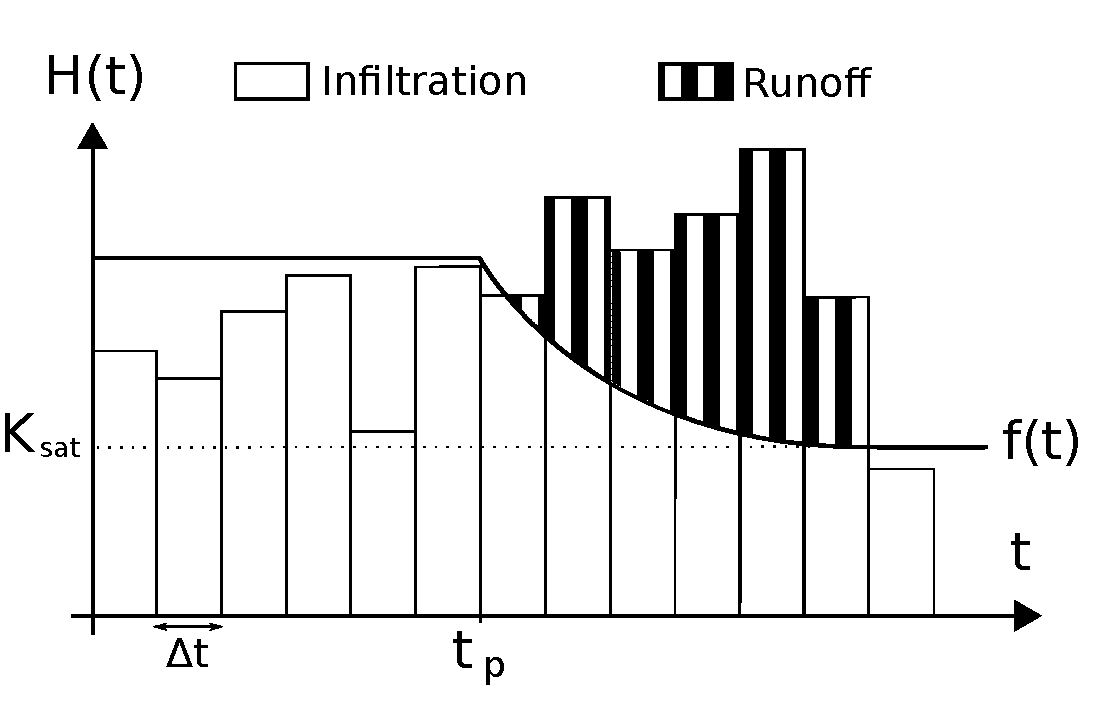
\includegraphics[width=8cm]{common/Separation_infiltration_ruissellement_MSeytoux.pdf}
\begin{equation}
\label{MSeytoux}
\begin{array}{l}
F(t) - F_p - \left(S_f + F_p \times \left(1 - \frac{1}{\beta_{MS}} \right) \right) \times ln \left(\frac{S_f + F(t)}{S_f+F_p} \right)\\
\\
 = \frac{K_s \times (t - t_p)}{\beta_{MS}}
\end{array}
\end{equation}


where $F_p$ is the cumulative infiltration when ponding occurs ($m$), $\beta_{MS}$ is the viscous correction parameter ($-$) ranged between 1 and 1,7 and usually taken equal to 1,3 \cite{MorelS1984}, $K_s$ is the saturated hydraulic conductivity ($m/s$). $K_s$ is a distributed parameter on surface units but it can be time variable as a function of soil practice and rainfall.\\

The parameter $S_f$ is a factor composed of storage and suction ($m$). This factor is calculated with the equation \ref{Sf_equation} which is an approximation of the ``suction head / water content'' relation curve $\phi(\theta)$, hereafter.\\

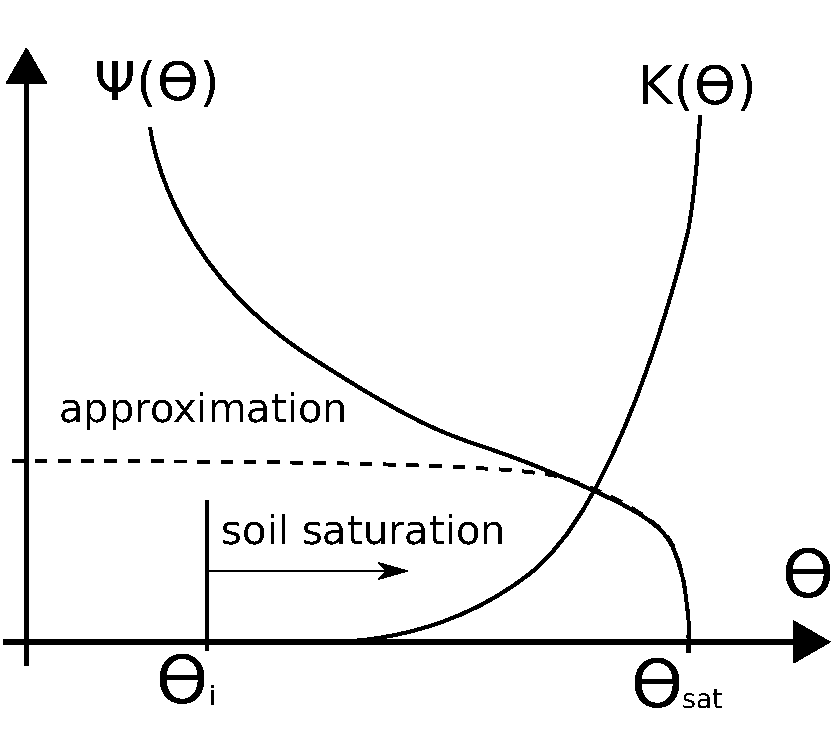
\includegraphics[width=8cm]{common/Sf_approximation.pdf}
\begin{equation}
\label{Sf_equation}
S_f=(\theta_s-\theta_i)\times H_c \times \left(1-\frac{1}{3}\times \left( \frac{\theta_i-\theta_r}{\theta_s-\theta_r} \right) ^6 \right)
\end{equation}


where $Hc$ is the capillary height ($m$), $\theta_s$  is the volumetric soil water content at saturation ($m\up3/m\up3$), $\theta_r$ is the volumetric residual soil water content ($m\up3 /m\up3$) and $\theta_i$ is the initial water content in the top surface layer ($m\up3 /m\up3$). This calculation is done once at the beginning of the simulation.\\

To determine the cumulative infiltration $F(t)$ at every time step, the function realizes iterations to satisfy the equation \ref{MSeytoux}. The parameter $ResStep$ ($m$) characterises the accuracy of calculated cumulative infiltration value. The smaller this parameter is, the more accurate the value $F$ is. However, simulation duration is higher because of the greater number of iteration steps.


\subsection{Calculation of infiltration and runoff}
Then, produced variables are calculated as following :\\

\hspace{-0.53cm} if $t \le t_p$ : \ \ \ \begin{equation}
\left\{ \begin{array}{l}
   I = H\\
   R = 0
  \end{array}
\right.
\end{equation}\\
\vspace{-0.5mm}
if $t > t_p$ : \ \ \ \begin{equation}
\left\{ \begin{array}{l}
   I = F(t) - F(t-1)\\
   R = H - \left(F(t) - F(t-1) \right)
  \end{array}
\right.
\end{equation}

where $I$ is the infiltrated water height ($m$), $R$ is the runoff water height on SU ($m$), $F$ is the cumulative infiltration ($m$) at time $t$, and $H$ is the water height at the top of the surface unit ($m$) calculated in equation \ref{HeightSU}.\\

We could note that once $t_p$ is reached, the soil cannot be ``unsaturated''. Therefore, the ``\englishname'' should be only used at the scale of a rain event.\\

Some examples of use are available in the paper of Morel-Seytoux \cite{MorelS1984}, Chahinian \cite{Chahinian2004b} and in thesis of Chahinian \cite{Chahinian2004} and Ghesquière \cite{Ghesquiere2008}.
}
  {\subsection{Calcul de la hauteur d'eau à séparer}
Dans un premier temps, la fonction va calculer la hauteur d'eau présente à la surface de l'unité. Elle se compose de la pluie $P$ (en $m$) ainsi que du débit de ruissellement $Q_{SU}(t-1)$ (en $m\up3/s$) provenant des éventuelles SU situées en amont et calculé au pas de temps précédent.

\begin{equation}
\label{HeightSU}
H = P + \sum_{SU_{up}} \left( \frac{Q_{SU}(t-1) \times \Delta t}{A_{SU}} \right)
\end{equation}


où $H$ est la hauteur d'eau présente à la surface de la SU ($m$), $\Delta t$ est le pas de temps de simulation ($s$), et $A_{SU}$ est la surface de l'unité sur laquelle est effectué le calcul ($m\up2$).


\subsection{Calcul de l'infiltrabilité}
La fonction de production de Morel-Seytoux \cite{MorelS1978} est une adaptation des hypothèses de Green et Ampt \cite{Green1911}. L'hypothèse majeure est la forme rectangulaire du front d'infiltration dans le sol, comme schématisé dans la figure ci-dessous. Le modèle a ensuite été adapté à la structure de MHYDAS par Moussa et al. \cite{Moussa2002}.\\

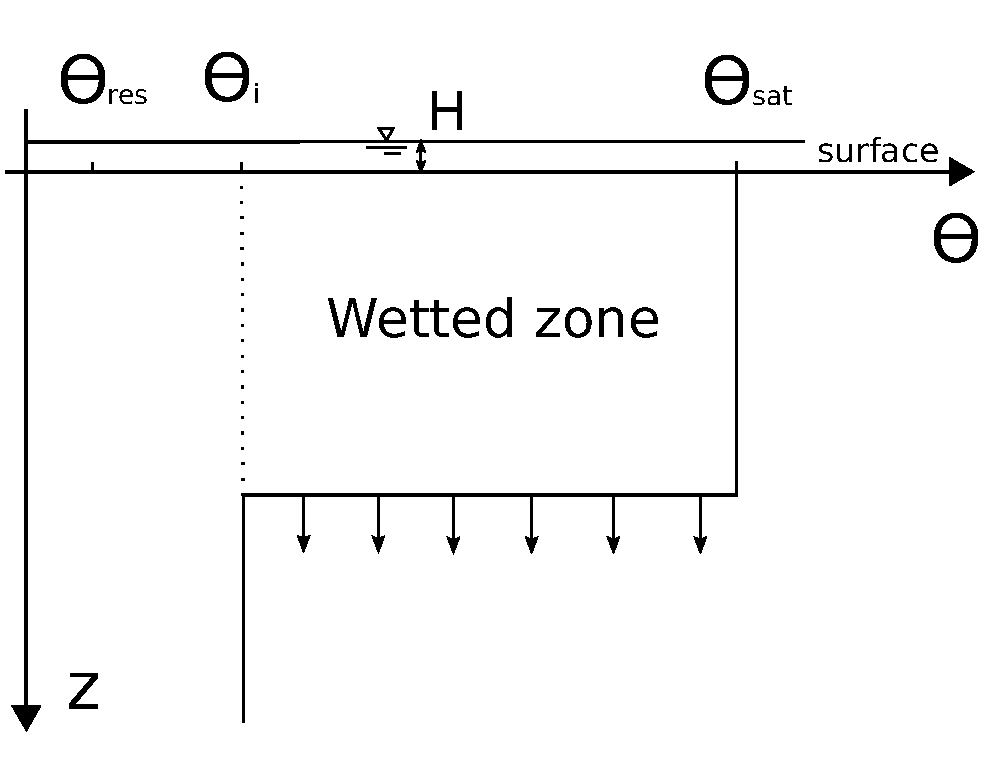
\includegraphics[width=8cm]{common/Green_Ampt_humidity.pdf}\\

Le ruissellement ne peut être observé que si le stock d'eau dans la couche superficielle du sol est à saturation. Ce temps caractéristique est appelé ``temps de flaquage''. Le modèle situe donc le début de l’infiltration maximale en fonction du temps de flaquage $t_p$ : lorsque $t < t_p$ toute la pluie est transformée en infiltration et quand $t > t_p$ il y a production de ruissellement selon l'équation \ref{MSeytoux}. Ce comportement peut être schématisé de la façon suivante avec l'infiltrabilité $f(t)$ ($m/s$) qui diminue au cours du temps à partir de $t_p$ pour tendre vers la conductivité hydraulique à saturation $K_{sat}$.\\

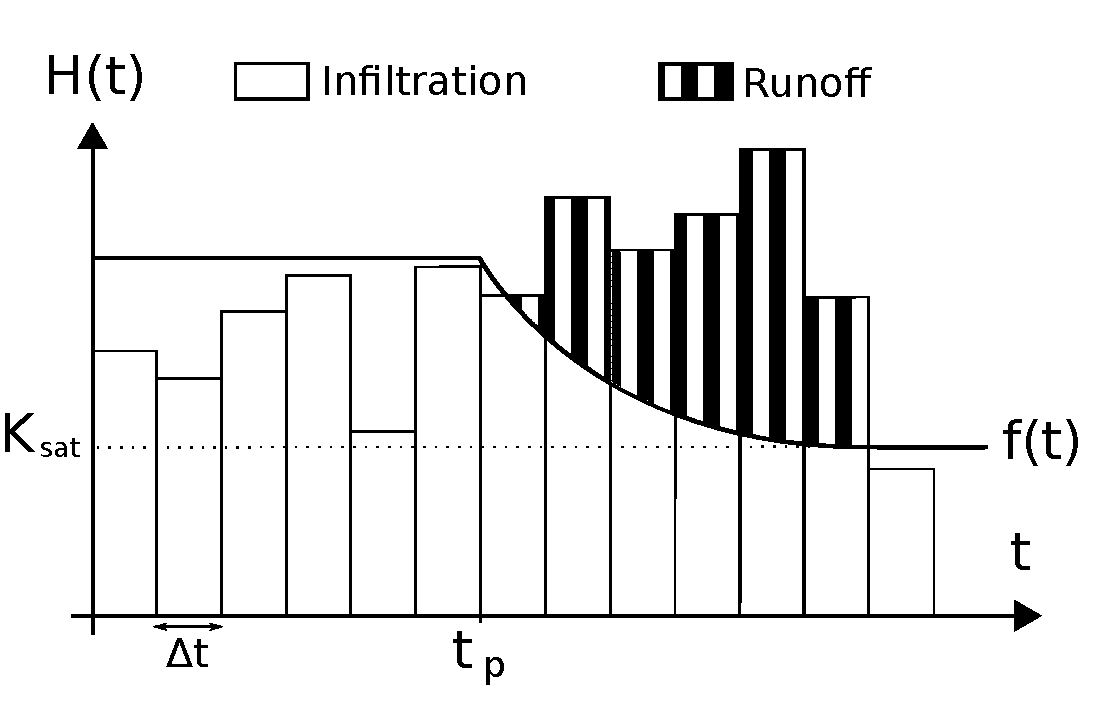
\includegraphics[width=8cm]{common/Separation_infiltration_ruissellement_MSeytoux.pdf}
\begin{equation}
\label{MSeytoux}
\begin{array}{l}
F(t) - F_p - \left(S_f + F_p \times \left(1 - \frac{1}{\beta_{MS}} \right) \right) \times ln \left(\frac{S_f + F(t)}{S_f+F_p} \right)\\
\\
 = \frac{K_s \times (t - t_p)}{\beta_{MS}}
\end{array}
\end{equation}


où $F(t)$ est l'infiltration cumulée au pas de temps $t$ ($m$) et l'intégrale de $f(t)$ représenté sur la figure ci-dessus, $F_p$ est l’infiltration cumulée à $t$ = $t_p$ ($m$), $\beta_{MS}$ est le coefficient de correction visqueuse ($-$) compris entre 1 et 1.7 et généralement pris égal à 1.3 \cite{MorelS1984}, et $K_s$ est la conductivité hydraulique à saturation ($m/s$). $K_s$ est un paramètre distribué sur les unités de surface mais il peut également être variable dans le temps en fonction du travail du sol notamment.\\

Le paramètre $S_f$ ($m$) est un facteur composé de stockage et de succion. L'équation \ref{Sf_equation} qui permet de calculer ce facteur est une approximation de la courbe d'évolution de la hauteur de succion en fonction de la teneur en eau du sol $\phi(\theta)$, ci-après.\\

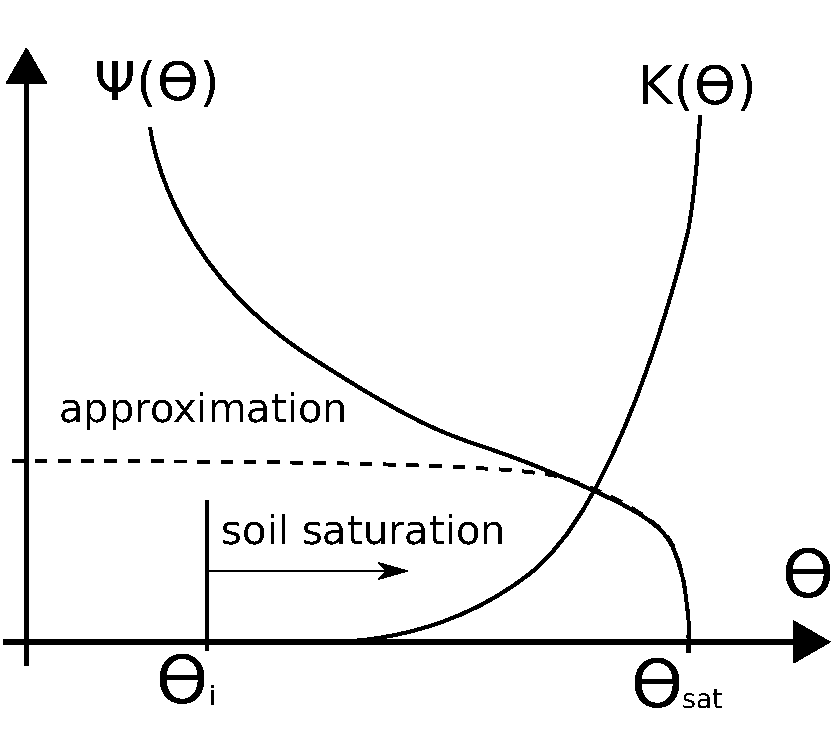
\includegraphics[width=8cm]{common/Sf_approximation.pdf}
\begin{equation}
\label{Sf_equation}
S_f=(\theta_s-\theta_i)\times H_c \times \left(1-\frac{1}{3}\times \left( \frac{\theta_i-\theta_r}{\theta_s-\theta_r} \right) ^6 \right)
\end{equation}


où $Hc$ est la poussée capillaire ($m$), $\theta_s$ est la teneur en eau à saturation ($m\up3 /m\up3$), $\theta_r$ est la teneur en eau résiduelle ($m\up3 /m\up3$) et $\theta_i$ est l’humidité initiale de la couche de surface ($m\up3 /m\up3$). Ce calcul est effectué une seule fois en début de simulation.\\

Pour déterminer l'infiltration cumulée $F(t)$ à chaque pas de temps, la fonction réalise des itérations afin de satisfaire l'équation \ref{MSeytoux}. Le paramètre $ResStep$ (en $m$) traduit la précision de la valeur d'infiltration cumulée calculée. Plus ce paramètre est faible, plus la valeur de $F$ est précise mais plus grand est le nombre d'itérations et donc plus la durée de la simulation sera longue.


\subsection{Calcul de l'infiltration et du ruissellement}
Les variables produites par la fonction sont ensuite calculées de la manière suivante :\\

\hspace{-0.53cm} si $t \le t_p$ : \ \ \ \begin{equation}
\left\{ \begin{array}{l}
   I = H\\
   R = 0
  \end{array}
\right.
\end{equation}\\
\vspace{-0.5mm}
si $t > t_p$ : \ \ \ \begin{equation}
\left\{ \begin{array}{l}
   I = F(t) - F(t-1)\\
   R = H - \left(F(t) - F(t-1) \right)
  \end{array}
\right.
\end{equation}

où $I$ est la hauteur d'eau infiltrée ($m$), $R$ est la hauteur d'eau qui ruisselle à la surface de la SU ($m$), $F$ est l'infiltration cumulée ($m$) au temps $t$, et $H$ est la hauteur d'eau à la surface de la SU ($m$) calculée par l'équation \ref{HeightSU}.\\

La fonction de Morel-Seytoux situant le début du ruissellement à partir du temps de flaquage, une fois que $t_p$ est atteint, le sol ne peut pas être ``désaturé''. C'est pour cette raison que cette fonction ne peut être utilisée qu'à l'échelle événementielle.\\

Des exemples d'utilisation sont disponibles dans la publication de Morel-Seytoux \cite{MorelS1984} et Chahinian \cite{Chahinian2004b} ainsi que dans les thèses de Chahinian \cite{Chahinian2004} et Ghesquière \cite{Ghesquiere2008}.
}


%******************************
% Functional description
\iflanguage{english}{\section{Functional description}}{\section{Notice d'utilisation}}
\iflanguage{english}{\subsection{Function name}
The name (fileID) of the simulation function is \texttt{\FileID}.


\subsection{Function parameters}
The function ``\englishname'' must be used with the following parameter :
\vspace{1em}

\hspace{-0.5cm}
\begin{tabular}{|llcc|}
 \hline
\it Symbol & \it Name & \it Value range & \it Unit \\
 \hline
$Res Step$ & \texttt{\ParamA} & $>0$ & $m$ \\
\hline
\end{tabular} 
\vspace{1em}

Thus, the correct syntax to use in the \texttt{model.xml} file is illustrated hereafter :

\begin{small}
\begin{verbatim}
<function fileID="water.surf-uz.runoff
          -infiltration.mseytoux">
    <param name="resstep"
           value="0.000005" />
</function>
\end{verbatim}
\end{small}



\subsection{Unit properties required}
Some of the soil properties are required. These are described in the following table :
\vspace{1em}

\hspace{-0.5cm}
\begin{tabular}{|llcc|}
 \hline
\it Symbol &\it Name & \it Value range & \it Unit \\
 \hline
$K_s$ & \texttt{\PropDisA} & $\geq 0$ & $m/s$ \\
$\theta_r $ & \texttt{\PropDisB} & $0 \le \theta_r \le 1$ & $m\up{3}/m\up{3}$ \\
$\theta_s$ & \texttt{\PropDisC} & $0 \le \theta_s \le 1$ & $m\up{3}/m\up{3}$ \\
$\beta_{MS}$ & \texttt{\PropDisD} & $>0$ & $-$ \\
$H_c$ & \texttt{\PropDisE} & $\geq 0$ & $m$ \\
$A_{SU}$ & \texttt{\PropDisF} & $>0$ & $m\up2$ \\
\hline
\end{tabular}
\vspace{1em}

The condition $\theta_r \le \theta_s$ must be verified.\\



\subsection{Initial conditions}
The function ``\englishname`` requires an initial condition which is located in the \texttt{SUini.ddata.xml} file.
\vspace{1em}

\hspace{-0.5cm}
\begin{tabular}{|llcc|}
 \hline
\it Symbol & \it Name & \it Value range & \it Unit \\
 \hline
$\theta_i$ & \texttt{\InitA} & $0 \le \theta_i \le 1$ & $m\up{3}/m\up{3}$ \\
\hline
\end{tabular} 
\vspace{1em}

The condition $\theta_r \le \theta_i \le \theta_s$ must be verified.\\



\subsection{Variables}
Variables produced, required and updated by this function are listed hereafter :
\vspace{1em}

\hspace{-0.5cm}
\begin{tabular}{|lll|}
 \hline
\it Symbol & \it Name & \it Unit \\
 \hline
$R$ & \texttt{\VarProdA} & $m$ \\
$I$ & \texttt{\VarProdB} & $m$ \\
$Q_{SU}$ & \texttt{\VarUsedA} & $m\up{3}/s$ \\
$K_s$ & \texttt{\VarUsedB} & $m/s$ \\
$P$ & \texttt{\VarRequirA} & $m$ \\
\hline
\end{tabular} 
\vspace{1em}
}
  {\subsection{Nom de la fonction}
Le nom (fileID) de la fonction de simulation est \texttt{\FileID}.

\subsection{Paramètres de la fonction}
La ``\frenchname'' doit être utilisée et renseignée avec le paramètre suivant :\\


\hspace{-0.5cm}
\begin{tabular}{|llcc|}
 \hline
\it Symbole & \it Nom & \it Valeurs & \it Unité \\
 \hline
$Res Step$ & \texttt{\ParamA} & $>0$ & $m$ \\
\hline
\end{tabular} 
\vspace{1em}

La syntaxe correcte de déclaration d'utilisation de la fonction dans le fichier \texttt{model.xml} doit ressembler à l'exemple illustré ci-après :

\begin{verbatim}
<function fileID="water.surf-uz.runoff
          -infiltration.mseytoux">
    <param name="resstep"
           value="0.000005" />
</function>
\end{verbatim}


\subsection{Propriétés distribuées}
La ``\frenchname'' requiert les propriétés distribuées suivantes :
\vspace{1em}

\hspace{-0.5cm}
\begin{tabular}{|llcc|}
 \hline
\it Symbole & \it Nom & \it Valeurs & \it Unité \\
 \hline
$K_s$ & \texttt{\PropDisA} & $\geq 0$ & $m/s$ \\
$\theta_r $ & \texttt{\PropDisB} & $0 \le \theta_r \le 1$ & $m\up{3}/m\up{3}$ \\
$\theta_s$ & \texttt{\PropDisC} & $0 \le \theta_s \le 1$ & $m\up{3}/m\up{3}$ \\
$\beta_{MS}$ & \texttt{\PropDisD} & $>0$ & $-$ \\
$H_c$ & \texttt{\PropDisE} & $\geq 0$ & $m$ \\
$A_{SU}$ & \texttt{\PropDisF} & $>0$ & $m\up2$ \\
\hline
\end{tabular} 
\vspace{1em}

La condition $\theta_r \le \theta_s$ devra être vérifiée.\\


\subsection{Conditions initiales}
Pour chaque SU, une condition initiale est nécessaire et doit être présente dans le fichier \texttt{SUini.ddata.xml}. Cette condition initiale est la suivante :
\vspace{1em}

\hspace{-0.5cm}
\begin{tabular}{|llcc|}
 \hline
\it Symbole & \it Nom & \it Valeurs & \it Unité \\
 \hline
$\theta_i$ & \texttt{\InitA} & $0 \le \theta_i \le 1$ & $m\up{3}/m\up{3}$ \\
\hline
\end{tabular} 
\vspace{1em}

La condition $\theta_r \le \theta_i \le \theta_s$ devra être vérifiée.\\


\subsection{Variables}
Les variables produites, utilisées et requises par cette fonction sont listées dans le tableau ci-après :
\vspace{1em}

\hspace{-0.5cm}
\begin{tabular}{|lll|}
 \hline
\it Symbole & \it Nom & \it Unité \\
 \hline
$R$ & \texttt{\VarProdA} & $m$ \\
$I$ & \texttt{\VarProdB} & $m$ \\
$Q_{SU}$ & \texttt{\VarUsedA} & $m\up{3}/s$ \\
$K_s$ & \texttt{\VarUsedB} & $m/s$ \\
$P$ & \texttt{\VarRequirA} & $m$ \\
\hline
\end{tabular} 
\vspace{1em}}

%******************************
% References
\bibliography{./common/water.surf-uz.runoff-infiltration.mseytoux.bib}

%******************************
% Appendices
\end{multicols}

%\clearpage

\begin{multicols}{2}
